\documentclass[11pt]{article}
\usepackage[utf8]{inputenc}  % gebruik de juiste 'character encoding'
\usepackage[dutch]{babel}    % definitie van de taal (Engels is de standaard)
\usepackage{hyperref}        % geef URLs netjes weer
\usepackage{booktabs}		 % mooiere tabellen
\usepackage{a4wide}          % papierformaat en marges
\usepackage{graphicx} 		 % Invoegen van plaatjes , ref: https://nl.sharelatex.com/learn/Inserting_Images
\usepackage{listings}
\usepackage{wrapfig}
\graphicspath{ {images/} }   % zet het pad voor de plaatjes
\pagestyle{plain}            % zet alleen paginanummering aan
% titel en auteur van het document
\title{Plan van Aanpak Project Domotica 1.2}

 \date{} % de datum van het document 
% einde definities; start van de tekst
\begin{document}
\thispagestyle{empty}
\maketitle %Maak het titelblad

\begin{figure}[h]
	\centering
	
\includegraphics[width=\textwidth]{inholland}
\end{figure}

\vspace{20mm} %ruimte creëren tussen figuur en opdrachtgever

\centering Dit project is in opdracht van Hogeschool INHolland.\\ Gemaakt in \LaTeX 

	\vspace{10mm}

\begin{tabular} {l c c} %https://nl.sharelatex.com/learn/Tables#!#Tables_with_fixed_length
	
	Tycho Meijeren & 616047& 616047@student.INholland.nl\\
	
	Timothy van der Steenhoven & 522397 & 522397@student.INholland.nl\\
	
	Niels Turenhout & 614314 & 614314@student.INholland.nl
\end{tabular}


\newpage

\tableofcontents
\thispagestyle{empty}

\newpage
\section{Achtergrond}

\paragraph{}
\begin{flushleft}
In dit hoofdstuk komt, zoals de titel al aangeeft, de achtergrond van het project aan bod.
De achtergrond zal bestaan uit een korte uitleg over de opdrachtgever van het project, de 
setting waarin het project uitgevoerd wordt en een korte uitleg over de vormgeving van het project.
\end{flushleft}
\paragraph{'Doomotica'}
\begin{flushleft}
	 Dit project heeft de naam Doomotica gekregen, vanwege een typfout en, omdat de projectgroep dat een passende naam vond. 
	De opdrachtgever van het project is Hogeschool INHolland te Alkmaar vanuit de opleiding Technische Informatica, 
	jaar 1 periode 2. De contactpersonen vanuit school zijn:\\
	\begin{tabular}{l l l}
		Docent TI & Sander Gieling & Sander.Gieling@inholland.nl\\
		Docent TI & Martijn Oldenburg & Martijn.Oldenburg@inholland.nl\\
		\end{tabular}
	\end{flushleft}

\paragraph{Setting}
\begin{flushleft}
	De setting van het project valt binnen de eisen die gesteld zijn in de projecthandleiding (Jeroen Bol \& Sander Gieling, 2015). De aanleiding van dit project is hierin ook te vinden: \\
	"Tijdens  deze  projectperiode  is  het  de  bedoeling  dat  studenten  in  het  kader  van
	Web	Development een werkende webapplicatie (gericht op het mobiele platform) ontwerpen
	en  realiseren." (Jeroen Bol \& Sander Gieseling, 2015)
\end{flushleft}

\begin{flushleft}
	Het bovenstaande citaat is breed. Om de vormgeving van het project helderder te krijgen volgen hier een aantal concrete eisen vanuit de handleiding: 
	\begin{itemize}
		\item Een web-applicatie die in een door de projectgroep gekozen browser gebruikt kan worden.
		\item Een communnicatie met door de projectgroep gekozen database voor het opslaan en uitlezen van gegevens server-side.
		\item Voor elk database systeem dient er een Entity-relationshipmodel (ERD) gemaakt te worden. 
		\item Voor elke functionaliteit dient er een Programma Structuur Diagram gemaakt te worden.
		\item De web-applicatie moet de geleverde domotica simulator 'DaHause' kunnen \underline{besturen}.
		\item De web-applicatie kan per gebruiker ingesteld worden door middel van een login-scherm.  
		\end{itemize}
	\newpage
	Naast de eisen vanuit de projecthandleiding voegt de projectgroep de volgende eisen toe:
	\begin{itemize}
		\item De web-applicatie heeft een muziekspeler / muziekbot.
		\item De web-applicatie wordt voorzien van een 'teller' die bijhoudt hoelang de gebruiker online is en geeft op basis hiervan een beloning.
		\item de web-applicatie heeft een Michael Bay modes.
	\end{itemize}
	\end{flushleft}

\begin{flushleft}
	Dit sluit het hoofdstuk 'Achtergrond' af. In dit hoofdstuk zijn alle grove eisen gesteld aan het project. In het volgende hoofdstuk 'De Opdracht' worden
	een aantal keuzes van de projectgroep toegelicht en gaat de projectgroep dieper in op de, hierboven genoemde, projecteisen
\end{flushleft}



\newpage
\section{De Opdracht}
\paragraph{Doelstelling}
\begin{flushleft}
	In het vorige hoofdstuk is de aanleiding aan bod geweest. Van deze aanleiding is een probleemstelling af te leiden:\\
	\vspace{2mm}
	\textit{Om voor periode 2, jaar 1 van de opleiding Technische Informatica te slagen dient er een web-applicatie ontworpen en gerealiseerd te worden inclusief onderzoeksverslag wat
	het gehele traject vastlegd. }\vspace{2mm} \\

    Van de probleemstelling is de volgende doelstelling te maken:
	
	\vspace{2mm}
	\textit{De projectgroep heeft aan het einde van periode 2 jaar 1 van de opleiding Technische Informatica een volledig project afgeleverd, inclusief een samenwerkingsovereenkomst, een Plan van Aanpak, een werkende gepersonaliseerde web-applicatie en een onderzoeksverslag.}\vspace{2mm}
	
	
	Naast dit hoofddoel gaat de projectgroep zich deze periode voornamelijk bezig houden met het correct uitvoeren van verschillende acties:
	\begin{itemize}
		\item Het opstellen van een samenwerkingsovereenkomst.
		\item Het maken van een Plan van Aanpak.
		\item Onderzoek doen.
		\item Het ontwerpen van een database door middel van een ERD.
		\item Het ontwerpen van een functie in de web-applicatie door middel van PSD's.
		\item Het realiseren van een database/functie op basis van gemaakte ontwerpen.
		\item Het schrijven van een onderzoeksverslag.
	\end{itemize}
\end{flushleft}

\begin{flushleft}
	Een aantal bovenstaande termen zijn onduidelijk. Wat is namelijk 'correct' onderzoek doen? Deze vragen worden gaande de periode beantwoord in de lessen van de opleiding.
	Uiteraard worden deze lessen zoveel mogelijk direct in het project geïmplementeerd.
\end{flushleft}
\paragraph{Projectresultaat}
\begin{flushleft}
	In het vorige hoofdstuk zijn de eisen van het project al aan bod gekomen. De eisen worden hier niet herhaald. In deze paragraaf wordt de vormgeving van het project besproken. 
	Het project heeft de volgende eindproducten (elk met een korte beschrijving):
	\begin{itemize}
		\item De web-applicatie: De webapplicatie is gemaakt in Microsoft ASP.NET 4.0 (2010). Vanuit de opleiding wordt versie 4.0 aangeraden, omdat verschillende toepassingen in Javascript foutmeldingen geven. \\ 
		Om de web-applicatie persoonlijk te maken kan elke gebruiker inloggen door verbinding te maken met de database en op die manier zijn/haar eigen URL's bereiken. Naast zijn/haar URL's staan er een paar spelletjes in Javascript (Quinstreet Enterprises, 1999).\\ Door achter elkaar enkele minuten in contact te blijven met de server krijgt de gebruiker hiervoor een beloning en die kan hij/zij dan inwisselen voor toegang tot spelletjes. \\De muziekbot bevindt zich ook op de pagina en zal muziek afspelen. Of de muziek van de server afkomstig is of van de gebruiker zelf, hangt af van de moeilijkheidsgraad van het implementeren ervan in de web-applicatie. \\
		De connectie en besturing van DaHaus zal plaatsvinden via 1 van de URL-tegeltjes. \\ \vspace{2mm}
		\begin{figure}
		\centering
		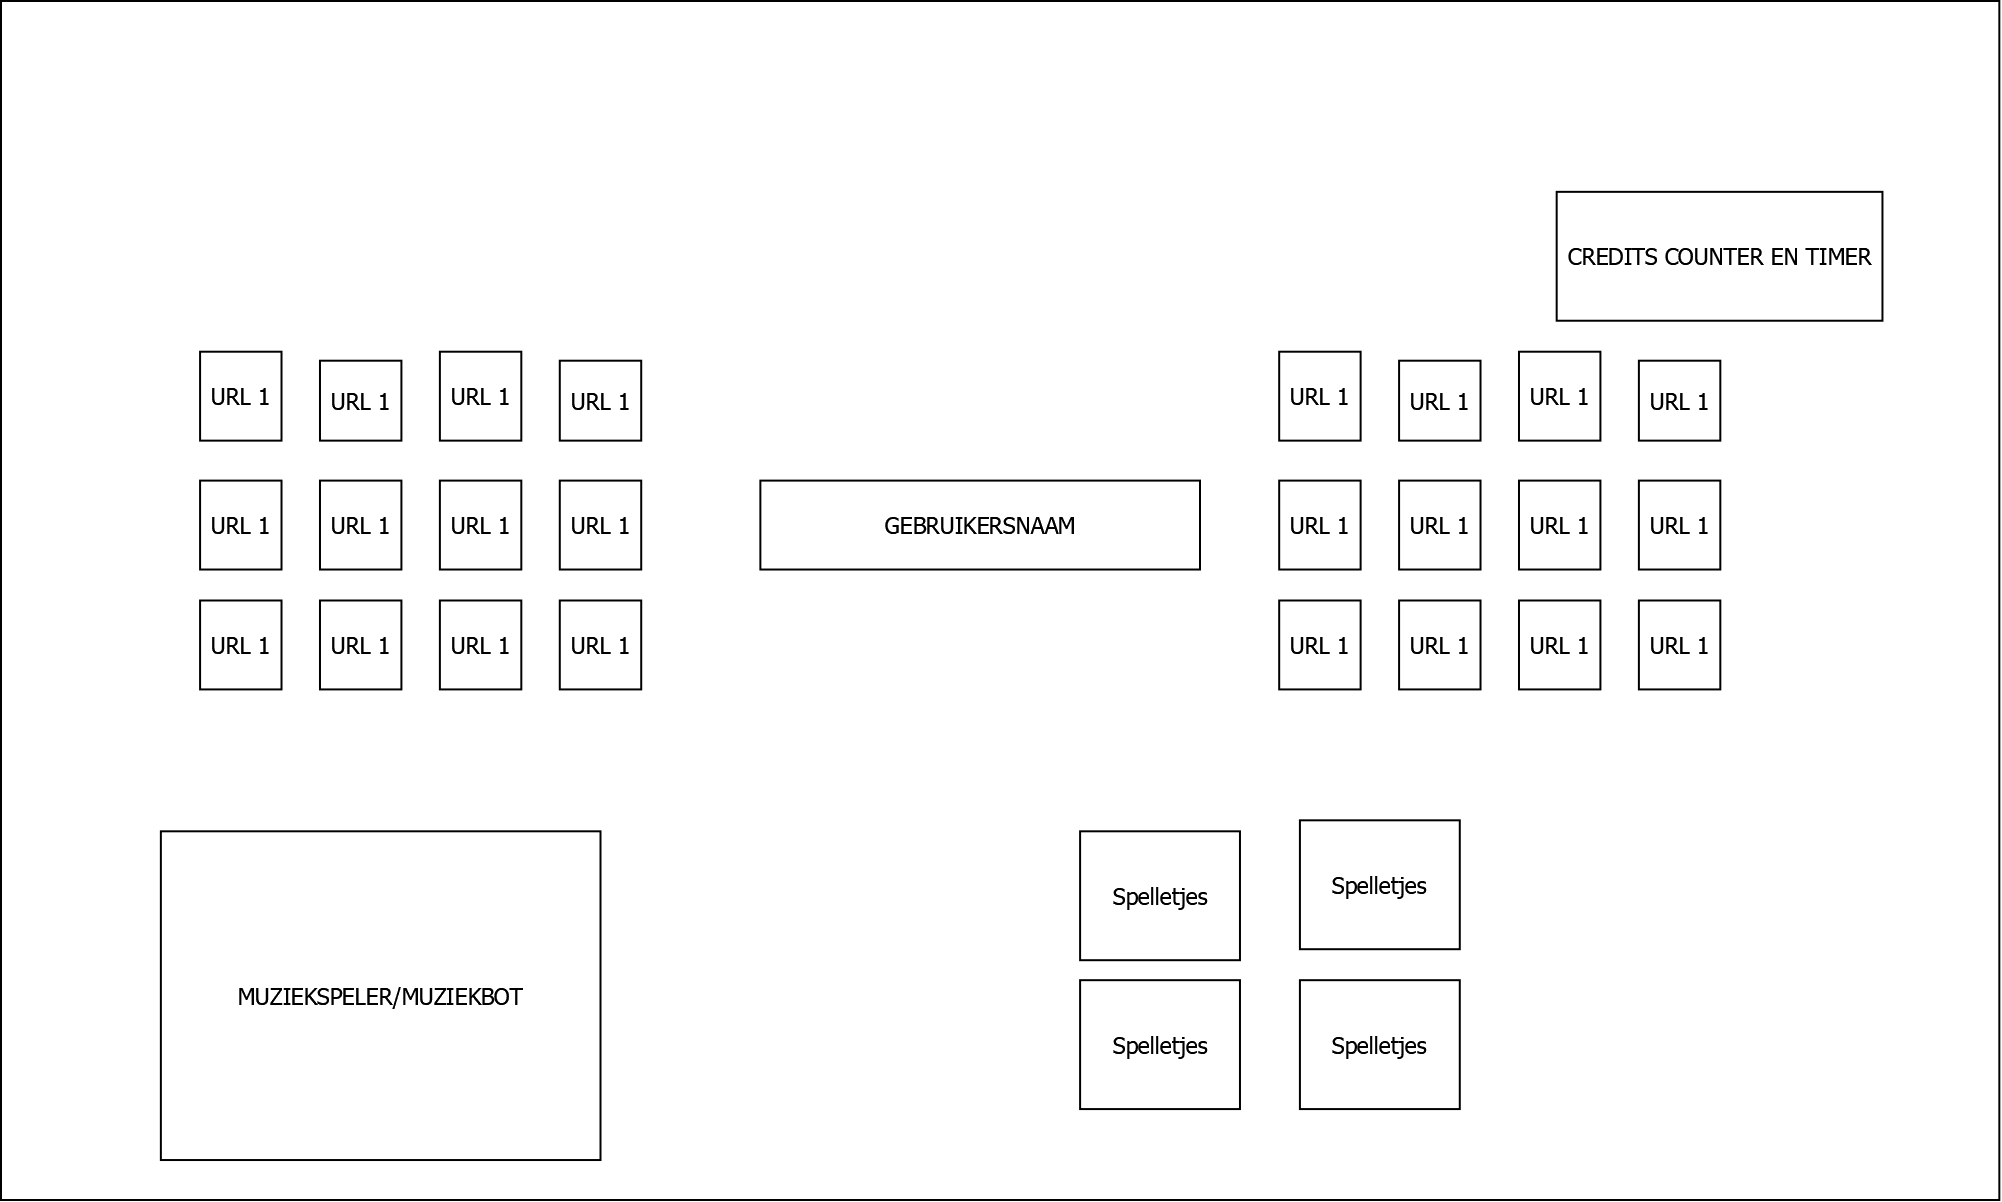
\includegraphics[width=\textwidth]{GUI} 
		\caption{Graphic User Interface}
		\end{figure}  \vspace{2mm}
		
		\item Het onderzoeksverslag: Het onderzoeksverslag gebruikt de richtlijnen die in het boek Projectmanagement (Roel Grit, 2015) worden besproken en het boek 'Onderzoek doen!' (Tom Fischer \& Mark Julsing, 2014). 
		Het verslag zal in \LaTeX geschreven worden. 
	\end{itemize}



\end{flushleft}
\newpage
\section{Projectactiviteiten}
\newpage
\section[Grenzen] {Grenzen van het project}
\newpage
\section{Deelproducten}
\newpage
\section{Kwaliteitsbewaking}

	

\begin{flushleft}
In hoofdstuk 2 'De Opdracht' staan de eisen van het project vanuit Hogeschool Inholland. Tijdens het projectassessment in januari 2018 zal het project beoordeelt worden door middel van een presentatie van het uiteindelijke product, een onderzoeksverslag en een peer-assessment.
\end{flushleft}
\paragraph{Communicatie}
\begin{flushleft}
De projectgroepcommuniceert met de contactpersoon vanuit school tijdens de lessen. Bij onduidelijkheden zal de het desbetreffende contact plaatsvinden via de e-mail. Elke dinsdag vergadert de projectgroep en wordt er overlegd met de contactpersoon of het project nog op schema ligt. 
\end{flushleft}
\paragraph{Controle}
\begin{flushleft}
De controle van het product zal eveneens elke dinsdag plaatsvinden tijdens de vergadering en wanneer groepsleden daar om vragen. Als een deelproduct klaar is, wordt het deelproduct eerst getest door groepsleden. Dit testen is gebaseerd op de volgende vragen:
\begin{itemize}
	\item Voldoet het deelproduct aan de eisen?
	\item Is dit deelproduct zo efficiënt/begrijpelijk mogelijk geschreven (code)?
	\item Hoe gaat de projectgroep dit implementeren in het hoofdprogramma?
\end{itemize}
\end{flushleft}
\paragraph{Softwaregebruik}
\begin{flushleft}
Alle software die gebruikt wordt is hieronder te vinden in de tabel (uitgebreide informatie is te vinden in de bronnenlijst):\\
\begin{tabular}[h]{l c c}
	Actie & Software & Versie\\ \hline
	Documenten & TeXstudio & 2.12.6\\ \hline 
	WebApplicatie & ASP.NET & 4.0\\ \hline
	Back-end code & C\# &  MS 2017\textsuperscript{A} \\ \hline
	IDE & Visual Studio 2017 & 15.4.3\\ \hline
	Testbrowser & Google Chrome & Versie 63.0.3239.84 (64-bit)\\ \hline
	Database maken & MS Acces & MS 2016\\ \hline
	ERD's maken & Dia & 0.97.2\\ \hline
	PSD's maken & Structorizer & 3.25-06\\ \hline
	Domotica connectie & DaHause & 1.0.0.1 \\ \hline
	
	\end{tabular}\\ 
\vspace{4mm}

\textsuperscript{A} Visual Studio 2017 geeft deze versie van C\# aan.
\end{flushleft}
\newpage
\section{De Projectorganisatie}
\newpage
\section{Planning}
\newpage
\section{Kosten en baten}
\newpage
\section{Risico's}
\newpage
\section{Bronnen}
\begin{itemize}
	\item Jeroen Bol \& Sander Gieling. (5 nov 2015). \textit{Projecthandleiding Domotica Technische Informatica, periode 2 jaar 1} (Inholland University of Applied Sciences, Alkmaar).  
	\item Tom Fischer \& Mark Julsing. (2014). \textit{Onderzoek doen!}, 2\textsuperscript{de} druk. (Noordhoff Uitgevers, Groningen/Houten).
	\item Roel Grit. (2015). \textit{Projectmanagement}, 7\textsuperscript{de} druk.(Noordhoff Uitgevers, Groningen/Houten).
	\item Microsoft. (2010). ASP.NET Framework (4.0) [Web applicatie software]. Opgevraagd van \url{https://docs.microsoft.com/en-us/aspnet/whitepapers/aspnet4/breaking-changes}
	\item Quinstreet Enterprises. (1999). The Javascript Source [Databank voor Javascript]. Opgevraagd van \url{http://www.javascriptsource.com/}
\end{itemize}




\section{Bijlagen}



















\end{document}